\subsection{Translational Controller}
SOMETHING ON THE RELATION BETWEEN ALL TRANSLATIONAL CONTROLLERS  DIAGRAM.
\fxnote{see the text}

%The translational control systems for x and y are structured as cascade, where the velocity and position are controlled in the inner and outer loop respectively.

\begin{figure}[H]
	\centering
	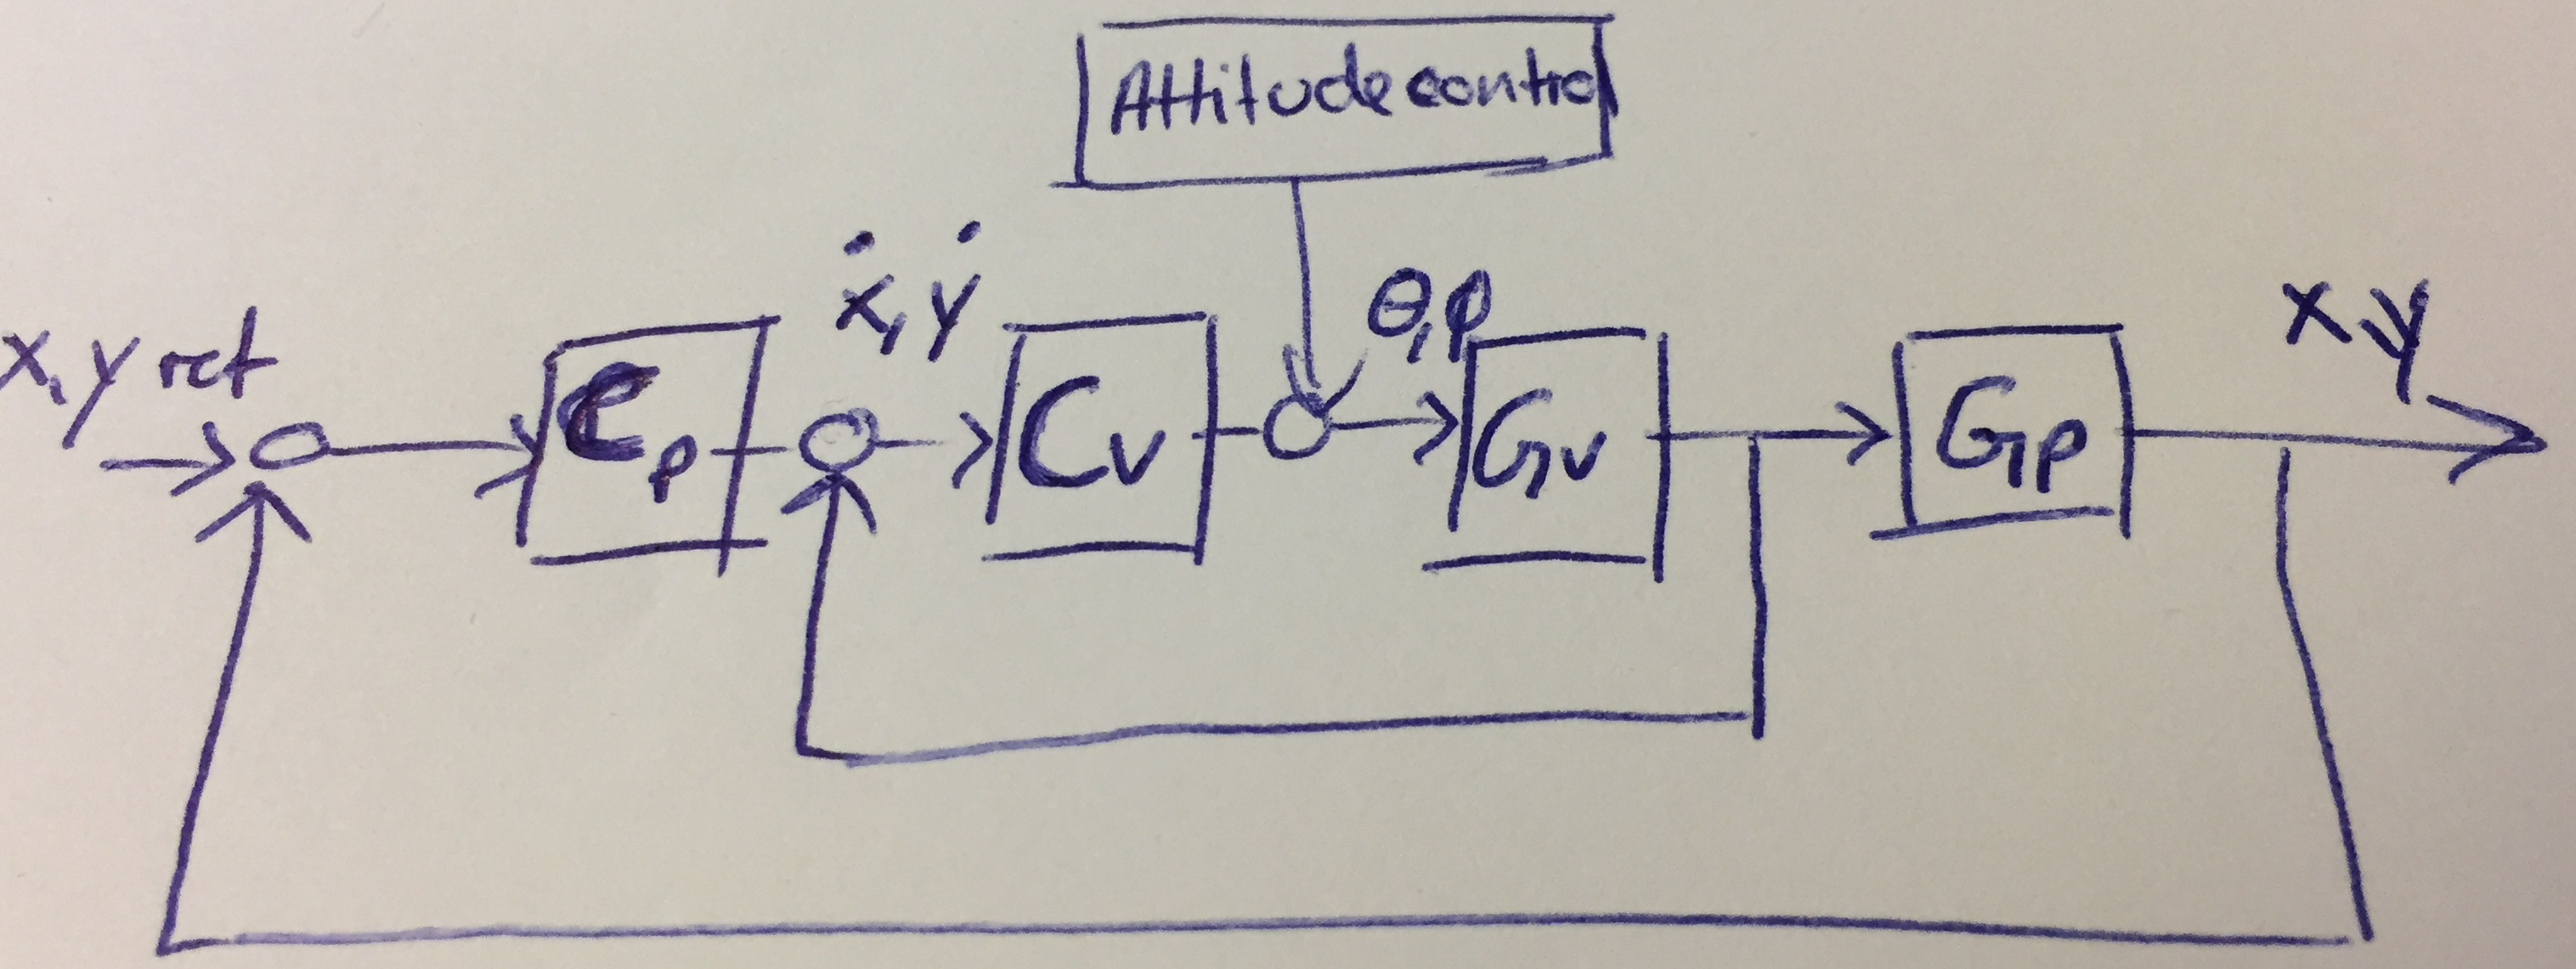
\includegraphics[scale=0.07]{figures/cascade_paper.png}
	\caption{Cascade loop for the translational controllers where the inner and outer loop control velocity and position respectively.}
	\label{fig:cascade}
\end{figure}
The x and y controller share similar properties as the output for each are an angle reference, namely $\theta_{ref}$ and $\phi_{ref}$ respectively.
Firstly the inner loop is designed followed by the outer loop.
The model equations derived previously, see Equation \ref{eq:AccelerationEqInertial1} and \ref{eq:AccelerationEqInertial2}, are Laplace transformed and put on transfer function in respect to the inner loop, yielding:
\begin{flalign}
    G_{\dot{x}_I}(s)&=\frac{\dot{x}_I (s)}{\theta (s)}=\frac{-k_{th} (\omega_1 ^2 + \omega_2 ^2 + \omega_3 ^2 + \omega_4 ^2)}{m\ s} \\
    G_{\dot{y}_I}(s)&=\frac{\dot{y}_I (s)}{\phi (s)}=\frac{k_{th}(\omega_1 ^2 + \omega_2 ^2 + \omega_3 ^2 + \omega_4 ^2)}{m\ s} 
\end{flalign}

\begin{where}
\va{G_{x_I}}{is the plant for the translational velocity in $x_I$ direction}{1}
\va{G_{y_I}}{is the plant for the translational velocity in $y_I$ direction}{1}
\end{where}
The plants are similar but with different signs. The controller design is carried out for the x translational velocity and applied to the y translational velocity afterwards.\\
A proportional controller is sufficient as the plant already has an integrator, that will eliminate a steady state error and output disturbances. The gain will be the same for both controllers, but must be negative for the x translational controller in order to compensate for its negative plant as this will otherwise be unstable in the closed loop.

The final proportional controllers are as follows:
\begin{align}
C_{\dot{x}I(s)= -0.19}\\
C_{\dot{y}I(s)= 0.19}
\end{align}
\begin{where}
    \va{G_{x_I}}{is the plant for the translational position in $x_I$ direction}{1}
    \va{G_{y_I}}{is the plant for the translational position in $y_I$ direction}{1}
\end{where}
The gain is designed such that it encounters a bandwidth that is three times lower than the attitude model to ensure minimum effect of disturbances. TO BE CONTINUED \fxnote{to be continued - Andrea}